\documentclass{ctexart}
\usepackage{Note}
\title{\textbf{Lab 1 报告}}
\author{蒋锦豪 2400011785}
\date{\today}
\begin{document}
\maketitle
\section*{Task 1: Image Dithering}
\subsection*{Uniform Random}
先调用{\codefont random}库生成均匀分布的随机数,然后对每个像素点进行处理,若加上随机数后大于0.5则设为黑色,否则设为白色.代码实现如下:
\begin{lstlisting}[language=C++]
void DitheringRandomUniform(
    ImageRGB &       output,
    ImageRGB const & input) {
    // your code here:
    std::random_device rd;
    std::mt19937 gen((unsigned int)rd());
    std::uniform_real_distribution<float> dis(-0.5,0.5);
    for (std::size_t x = 0; x < input.GetSizeX(); ++x)
        for (std::size_t y = 0; y < input.GetSizeY(); ++y) {
            glm::vec3 color = input.At(x, y);
            int graysacle = (color.r + dis(gen)) > 0.5 ? 1 : 0;
            output.At(x, y) = { graysacle, graysacle, graysacle, };
        }
}
\end{lstlisting}
效果图如下:
\begin{figure}[H]
    \centering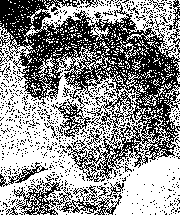
\includegraphics[scale=0.75]{figure/UniformRandom.png}
    \caption{Uniform Random Dithering的运行结果}
\end{figure}
\subsection*{Blue Noise Random}
将{\codefont input}和{\codefont noise}两张图像的像素值的平均值与$0.5$进行比较,若大于$0.5$则设为黑色,否则设为白色.实际运算时直接将像素值之和与$1$比较即可.代码实现如下:
\begin{lstlisting}[language=C++]
void DitheringRandomBlueNoise(
    ImageRGB &       output,
    ImageRGB const & input,
    ImageRGB const & noise) {
    // your code here:
    for (std::size_t x = 0; x < input.GetSizeX(); ++x)
        for (std::size_t y = 0; y < input.GetSizeY(); ++y) {
            glm::vec3 color_input = input.At(x, y);
            glm::vec3 color_noise = noise.At(x, y);
            int       graysacle   = (color_input.r + color_noise.r) > 1 ? 1 : 0;
            output.At(x, y)       = {
                graysacle, graysacle, graysacle, };
        }
}
\end{lstlisting}
效果图如下:
\begin{figure}[H]
    \centering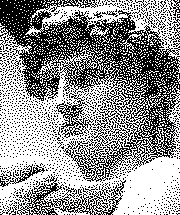
\includegraphics[scale=0.75]{figure/BlueNoise.png}
    \caption{Blue Noise Random Dithering的运行结果}
\end{figure}
\subsection*{Ordered}
将原图的像素值$i$扩大为$9i$,于是颜色取值范围变为$[0,9]$.将$9i$与$3\times3$的抖动矩阵{\codefont mat}的每个元素进行比较,如果大于该元素的值则将对应位置设为黑色,否则设为白色.代码实现如下:
\begin{lstlisting}[language=C++]
void DitheringOrdered(
    ImageRGB &       output,
    ImageRGB const & input) {
    // your code here:
    int mat[3][3] = {
        { 6, 8, 4 }, { 1, 0, 3 }, { 5, 2, 7 }
    };
    for (std::size_t x = 0; x < input.GetSizeX(); ++x)
        for (std::size_t y = 0; y < input.GetSizeY(); ++y) {
            glm::vec3 color = input.At(x, y);
            float     color_judge = color.r * 9;
            for (int i = 0; i < 3; i++) {
                for (int j = 0; j < 3; j++) {
                    int color_draw = color_judge >= mat[i][j] ? 1 : 0;
                    output.At(3 * x + i, 3 * y + j) = {
                        color_draw, color_draw, color_draw, };
                }
            }
        }
}
\end{lstlisting}
效果图如下:
\begin{figure}[H]
    \centering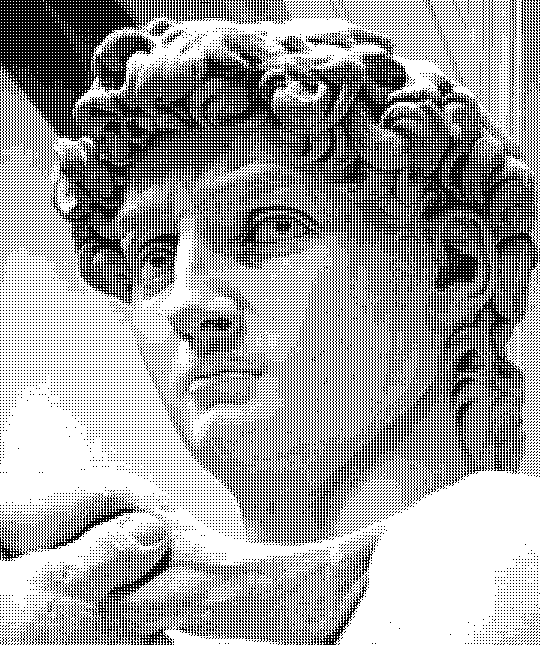
\includegraphics[scale=0.5]{figure/Ordered.png}
    \caption{Ordered Dithering的运行结果}
\end{figure}
\subsection*{Error Diffuse}
先将{\codefont input}的像素值存入一个二维数组{\codefont colormat}中,然后从左到右,从上到下遍历每个像素点,将{\codefont colormat}存储的像素值与0.5比较后将{\codefont output}对应位置的像素设为黑色或白色,并计算出误差{\codefont delta}.按照Floyd-Steinberg抖动矩阵和误差值{\codefont delta}在{\codefont colormat}中更新右方和下方的像素值;同时需要注意边界处像素的处理.代码实现如下:
\begin{lstlisting}[language=C++]
void DitheringErrorDiffuse(
    ImageRGB &       output,
    ImageRGB const & input) {
    // your code here:
    std::size_t                     row = input.GetSizeX(), col = input.GetSizeY();
    std::vector<std::vector<float>> colormat(row, std::vector<float>(col, 0));
    for (std::size_t x = 0; x < row; ++x) {
        for (std::size_t y = 0; y < col; ++y) {
            glm::vec3 color = input.At(x, y);
            colormat[x][y]  = color.r;
        }
    }
    for (std::size_t y = 0; y < col; ++y) {
        for (std::size_t x = 0; x < row; ++x) {
            int color       = colormat[x][y] > 0.5 ? 1 : 0;
            output.At(x, y) = {
                color, color, color, };
            float delta = colormat[x][y] - (colormat[x][y] > 0.5 ? 1 : 0);
            if (x < row - 1) { colormat[x + 1][y] += delta * 7 / 16; }
            if (y < col - 1) {
                colormat[x][y + 1] += delta * 5 / 16;
                if (x > 0) { colormat[x - 1][y + 1] += delta * 3 / 16; }
                if (x < row - 1) { colormat[x + 1][y + 1] += delta * 1 / 16; }
            }
        }
    }
}   
\end{lstlisting}
效果图如下:
\begin{figure}[H]
    \centering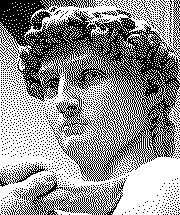
\includegraphics[scale=0.75]{figure/ErrorDiffuse.png}
    \caption{Error Diffuse Dithering的运行结果}
\end{figure}
\section*{Task 2 Image Filtering}
\subsection*{Blur}
使用$3\times3$的均值滤波器
\[\mat{K}=\dfrac19\begin{vmatrix}
    1&1&1\\
    1&1&1\\
    1&1&1
\end{vmatrix}\]
对图像进行滤波.具体实现时,遍历每个像素,将该像素及其周围8个像素的值相加后除以9即为滤波后的像素值.对于图像边缘的像素,如果越界则不计入求和和计数.代码实现如下:
\begin{lstlisting}[language=C++]
void Blur(
    ImageRGB &       output,
    ImageRGB const & input) {
    // your code here:
    std::size_t row = input.GetSizeX(), col = input.GetSizeY();
    for (std::size_t x = 0; x < row; ++x)
        for (std::size_t y = 0; y < col; ++y) {
            int ave_counter = 0;
            glm::vec3 color(0.0f, 0.0f, 0.0f);
            for (int i = -1; i <= 1; i++) {
                for (int j = -1; j <= 1; j++) {
                    if (x + i >= 0 && x + i < row && y + j >= 0 && y + j < col) {
                        ave_counter++;
                        color += input.At(x + i, y + j);
                    }
                }
            }
            output.At(x, y) = {
                color.r / ave_counter, color.g / ave_counter, color.b / ave_counter,
            };
        }
}
\end{lstlisting}
效果图如下:
\begin{figure}[H]
    \centering
\includegraphics[scale=0.4]{figure/Blur.png}
    \caption{Blur(使用Box Filter)的运行结果}
\end{figure}
\subsection*{Edge Detect}
使用Sobel算子
\[\mat{K}_x=\begin{vmatrix}
    -1&0&1\\
    -2&0&2\\
    -1&0&1
\end{vmatrix},\quad\mat{K}_y=\begin{vmatrix}
    1&2&1\\
    0&0&0\\
    -1&-2&-1
\end{vmatrix}\]
对图像进行滤波,然后以结果的均方根作为输出像素值.具体实现时,遍历每个像素,将该像素及其周围8个像素的值与$\mat{K}_x$和$\mat{K}_y$对应位置的值相乘后求和,结果分别记作{\codefont color\_x}和{\codefont color\_y},再对每个颜色通道分别计算它们的平方和开根号,结果即滤波后的像素值.对于图像边缘的像素,与\textbf{Blur}的处理方法相同,如果越界则不计入求和.代码实现如下:
\begin{lstlisting}[language=C++]
void Edge(
    ImageRGB &       output,
    ImageRGB const & input) {
    // your code here:
    float G_x[3][3] = {
        { -1.0f, 0.0f, 1.0f },
        { -2.0f, 0.0f, 2.0f },
        { -1.0f, 0.0f, 1.0f }
    };
    float G_y[3][3] = {
        {  1.0f,  2.0f,  1.0f },
        {  0.0f,  0.0f,  0.0f },
        { -1.0f, -2.0f, -1.0f }
    };
    std::size_t row = input.GetSizeX(), col = input.GetSizeY();
    for (std::size_t x = 0; x < row; ++x)
        for (std::size_t y = 0; y < col; ++y) {
            glm::vec3 color_x(0.0f, 0.0f, 0.0f);
            glm::vec3 color_y(0.0f, 0.0f, 0.0f);
            for (int i = -1; i <= 1; i++) {
                for (int j = -1; j <= 1; j++) {
                    if (x + i >= 0 && x + i < row && y + j >= 0 && y + j < col) {
                        glm::vec3 color_cur = input.At(x + i, y + j);
                        color_x += color_cur * G_x[i + 1][j + 1];
                        color_y += color_cur * G_y[i + 1][j + 1];
                    }
                }
            }
            output.At(x, y) = {
                sqrt(pow(color_x.r, 2) + pow(color_y.r, 2)),
                sqrt(pow(color_x.g, 2) + pow(color_y.g, 2)),
                sqrt(pow(color_x.b, 2) + pow(color_y.b, 2)),
            };
        }
}
\end{lstlisting}
效果图如下:
\begin{figure}[H]
    \centering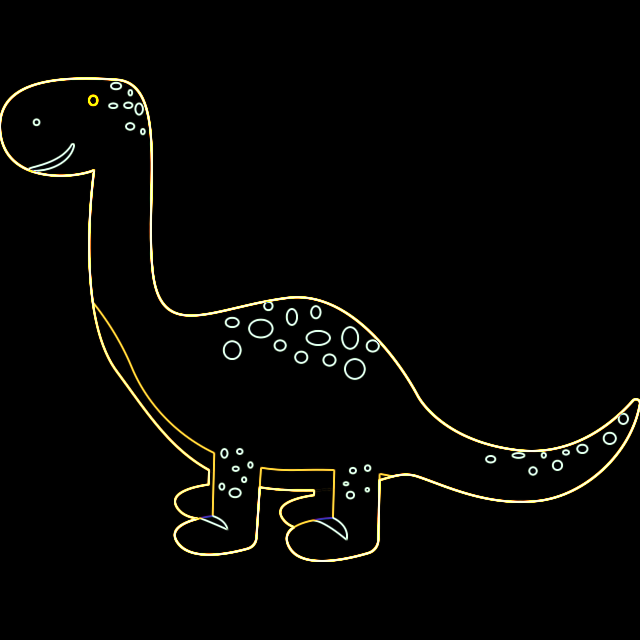
\includegraphics[scale=0.4]{figure/EdgeDetection.png}
    \caption{Edge Detect(使用Sobel Filter)的运行结果}
\end{figure}
\section*{Task 3: Inmage Inpainting}
采用任务指示中给出的记号,将修改前的图片记作$\vec{f}$,即传入的参数{\codefont inputFront},编辑量记作$\vec{g}$,编辑后的图像记作$\vec{f}+\vec{g}$,即需要输出的图片{\codefont output}中对应{\codefont inputFront}的区域.于是不难得出
\[\vec{g}=(\vec{f}+\vec{g})-\vec{f}=\text{{\codefont output}}-\text{{\codefont inputFront}}\]最终要求$\nabla^2\vec{g}=\mbf{0}$.按照Poisson Editing的思路,需要将设置边界处的$\vec{g}$,使得在边界上总有{\codefont output}与背景{\codefont inputBack}相同.于是边界部分的$\vec{g}$应当按
\[\vec{g}=\text{{\codefont output}}-\text{{\codefont inputFront}}=\text{{\codefont inputBack}}-\text{{\codefont inputFront}}\]
设置,该部分代码如下:
\begin{lstlisting}[language=C++]
// set boundary condition
for (std::size_t y = 0; y < height; ++y) {
    // set boundary for (0, y), your code: g[y * width] = ?
    g[y * width] = (glm::vec3) inputBack.At(offset.x, y + offset.y) - (glm::vec3) inputFront.At(0, y);
    // set boundary for (width - 1, y), your code: g[y * width + width - 1] = ?
    g[y * width + width - 1] = (glm::vec3) inputBack.At(offset.x + width - 1, y + offset.y) - (glm::vec3) inputFront.At(width - 1, y);
}
for (std::size_t x = 0; x < width; ++x) {
    // set boundary for (x, 0), your code: g[x] = ?
    g[x] = (glm::vec3) inputBack.At(x + offset.x, offset.y) - (glm::vec3) inputFront.At(x, 0);
    // set boundary for (x, height - 1), your code: g[(height - 1) * width + x] = ?
    g[(height - 1) * width + x] = (glm::vec3) inputBack.At(x + offset.x, offset.y + height - 1) - (glm::vec3) inputFront.At(x, height - 1);
}
\end{lstlisting}
效果图如下:
\begin{figure}[H]
    \centering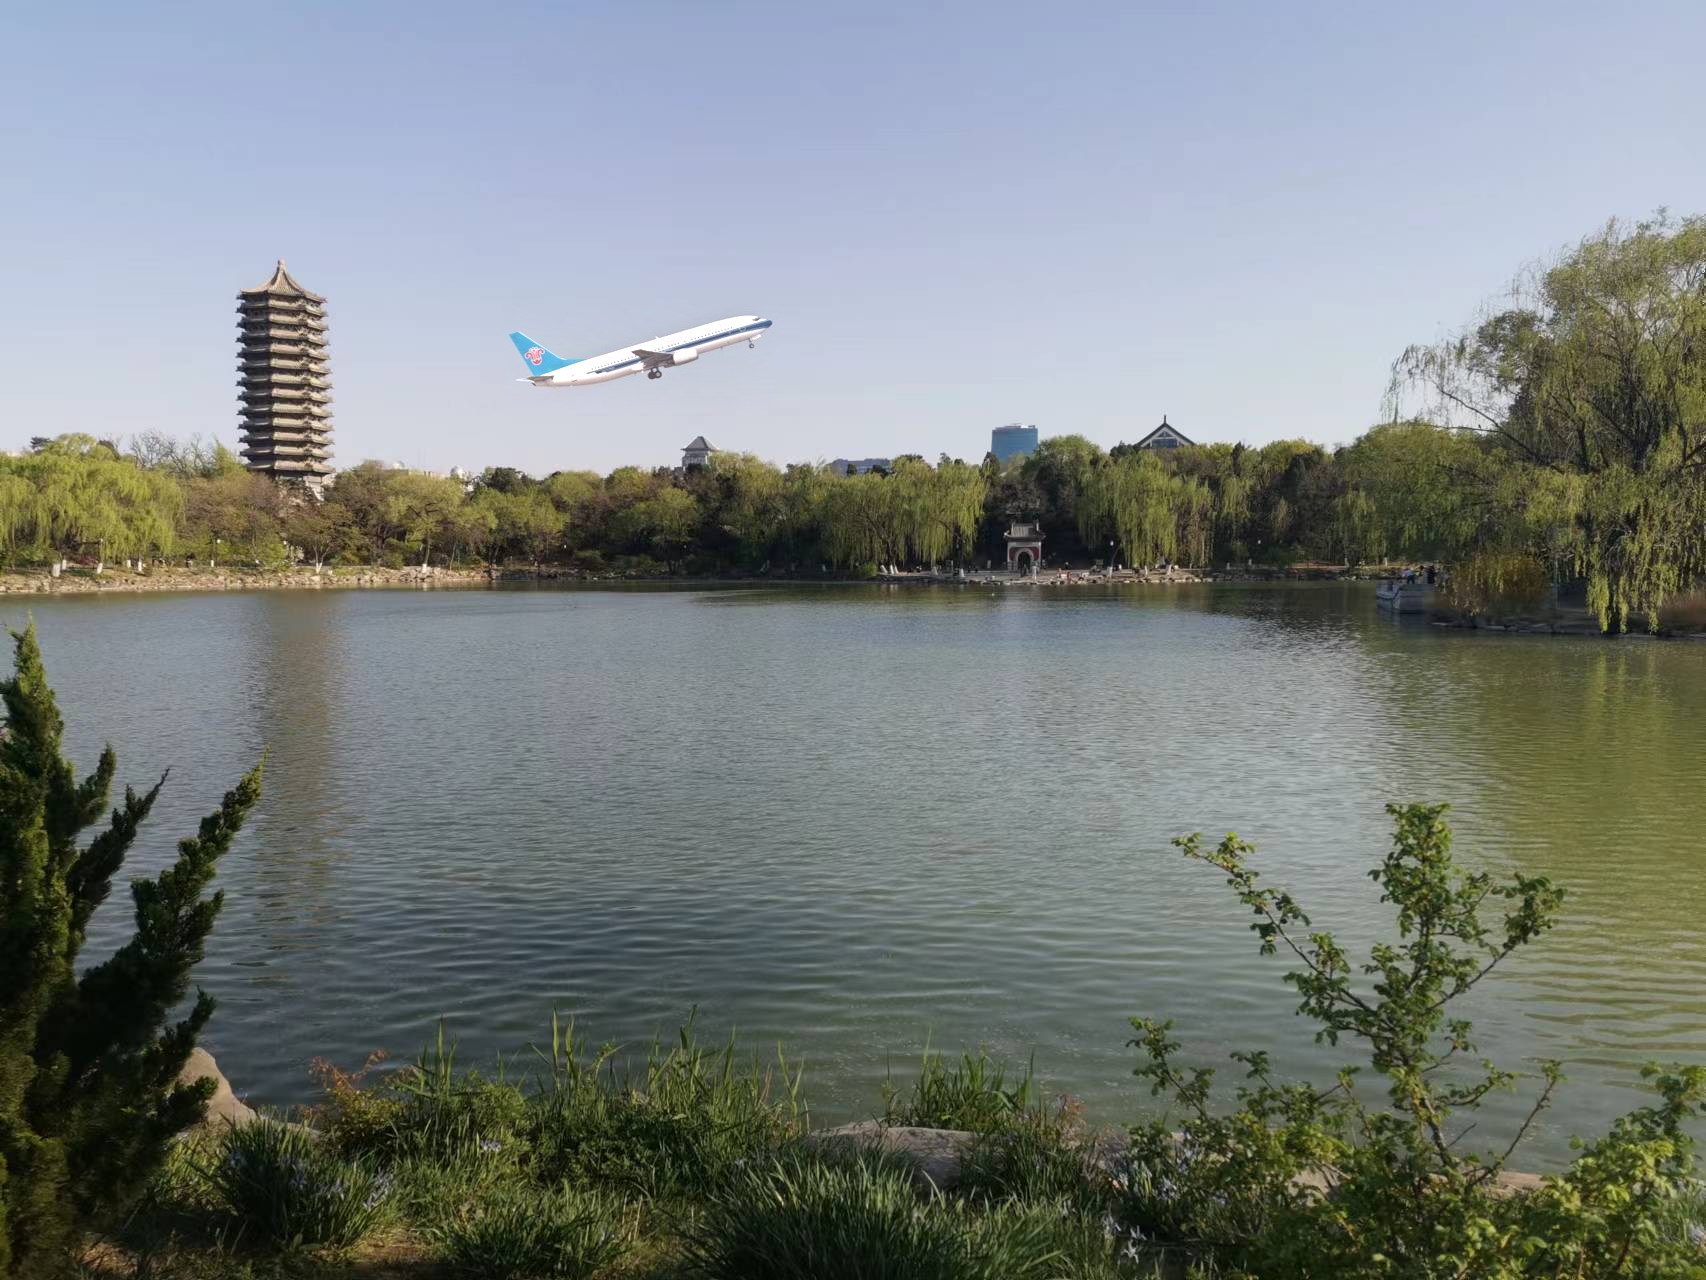
\includegraphics[scale=0.2]{figure/Inpainting.png}
    \caption{Image Inpainting的运行结果}
\end{figure}
\section*{Task 4: Line Drawing}
按照Bresenham算法实现直线绘制.具体实现时,先判断直线的斜率是否大于1,若是,则将{\codefont x0}与{\codefont y0}, {\codefont x1}与{\codefont y1}交换,并\textbf{在后续绘制时将横纵坐标互换回来};然后保证$\text{\codefont x0}\leqslant\text{\codefont x1}$,若不满足则交换两端点;接着按照Bresenham算法计算{\codefont dx}和{\codefont dy},以及判断函数{\codefont F}和{\codefont d};最后从{\codefont x0}遍历到{\codefont x1},每次根据决策参数{\codefont F}决定是否需要改变{\codefont y}(对{\codefont y}的增减取决于直线斜率的正负,在确定$\text{\codefont x1}>\text{\codefont x0}$的情况下,如果$\text{\codefont y1}>\text{\codefont y0}$说明斜率为正,每次将{\codefont y}加$1$;否则就每次将{\codefont y}减$1$.),并更新判断函数{\codefont F}.代码实现如下:
\begin{lstlisting}[language=C++]
    void DrawLine(
    ImageRGB &       canvas,
    glm::vec3 const  color,
    glm::ivec2 const p0,
    glm::ivec2 const p1) {
    // your code here:
    int x0 = p0.x, y0 = p0.y, x1 = p1.x, y1 = p1.y;
    int x, y, dx, dy, d, F, cx, cy;
    bool f = std::abs(x1 - x0) < std::abs(y1 - y0);
    if (f) { std::swap(x0, y0); std::swap(x1, y1); }
    if (x0 > x1) { std::swap(x0, x1); std::swap(y0, y1); }
    y  = y0; 
    dx = 2 * (x1 - x0); dy = 2 * std::abs(y1 - y0);
    d  = dy - dx; F  = dy - dx / 2;
    for (x = x0; x <= x1; x++) {
        cx = f ? y : x; cy = f ? x : y;
        canvas.At(cx, cy) = { color.r, color.g, color.b, };
        if (F < 0) {  F = F + dy; } 
        else { y += (y1 > y0) ? 1 : -1; F = F + d; }
    }
}
\end{lstlisting}
效果图如下:
\begin{figure}[H]
    \centering\subfigure[直线1]{
        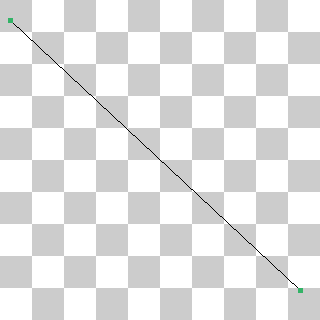
\includegraphics[scale=0.4]{figure/Line_1.png}
    }\quad
    \subfigure[直线2]{
        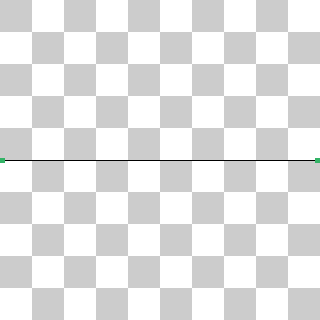
\includegraphics[scale=0.4]{figure/Line_2.png}
    }\quad
    \subfigure[直线3]{
        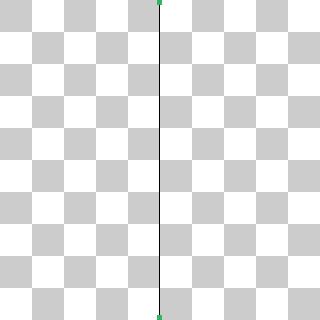
\includegraphics[scale=0.4]{figure/Line_3.png}
    }
    \caption{Line Drawing的运行结果}
\end{figure}
\section*{Task 5: Triangle Drawing}
按照扫描线算法实现三角形填充.具体实现时,先将三个顶点按横坐标从小到大排序,然后以位居中间的点为界分两段处理.对于左半段,先计算两条线段的斜率,然后从左到右遍历每列像素,按照DDA算法更新该列填充的的上下边界{\codefont ymin}和{\codefont ymax},并对该列上在上下边界之间的像素点进行填充;对于右半段,同理,只是从右到左遍历每个像素点.代码实现如下:
\begin{lstlisting}
    void DrawTriangleFilled(
    ImageRGB &       canvas,
    glm::vec3 const  color,
    glm::ivec2 const p0,
    glm::ivec2 const p1,
    glm::ivec2 const p2) {
    // your code here:
    int        x0 = p0.x, y0 = p0.y, x1 = p1.x, y1 = p1.y, x2 = p2.x, y2 = p2.y;
    float      ymin, ymax;
    float      k1, k2;
    if (x2 < x1) { std::swap(x1, x2); std::swap(y1, y2); }
    if (x1 < x0) { std::swap(x0, x1); std::swap(y0, y1); }
    if (x0 != x1 && x2 != x0) {
        ymin = 1.0 * y0; ymax = 1.0 * y0;
        k1 = 1.0 * (y1 - y0) / (x1 - x0); k2 = 1.0 * (y2 - y0) / (x2 - x0);
        if (k1 > k2) { std::swap(k1, k2); }
        for (int x = x0; x <= std::min(x1, x2); x++) {
            for (int y = std::round(ymin); y < ymax+0.5; y++) {
                canvas.At(x, y) = { color.r, color.g, color.b, };
            }
            ymin += k1; ymax += k2;
        }
    }
    if (x1 != x2 && x2 != x0) {
        ymin = 1.0 * y2; ymax = 1.0 * y2;
        k1 = 1.0 * (y1 - y2) / (x2 - x1); k2 = 1.0 * (y0 - y2) / (x2 - x0);
        if (k1 > k2) { std::swap(k1, k2); }
        for (int x = x2; x >= std::max(x1, x0); x--) {
            for (int y = std::round(ymin); y < ymax+0.5; y++) {
                canvas.At(x, y) = { color.r, color.g, color.b, };
            }
            ymin += k1; ymax += k2;
        }
    }
}
\end{lstlisting}
效果图如下:
\begin{figure}[H]
    \centering\subfigure[三角形1]{
        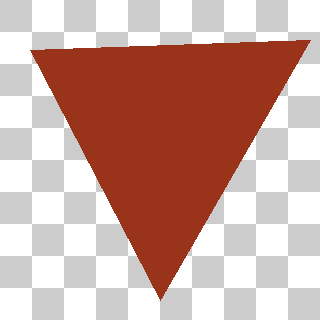
\includegraphics[scale=0.4]{figure/Triangle_1.png}
    }\quad
    \subfigure[三角形2]{
        
\includegraphics[scale=0.4]{figure/Triangle_2.png}
    }\quad
    \subfigure[三角形3]{
        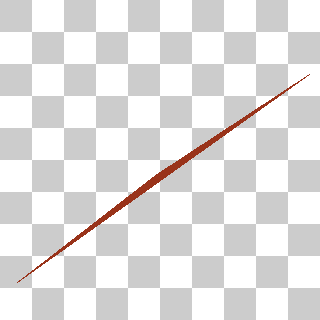
\includegraphics[scale=0.4]{figure/Triangle_3.png}
    }
    \caption{Triangle Drawing的运行结果}
\end{figure}
\section*{Task 6: Image Supersampling}
使用双线性插值对图像进行放大,然后对放大的图像进行均值滤波.具体实现时,先创建一个二维数组{\codefont colormatrix}存储放大后的图像的像素值,然后遍历放大后图像的每个像素点,计算出其在原图中对应的浮点坐标{\codefont (sx, sy)},并找出其周围的4个像素点{\codefont (x0, y0), (x1, y0), (x0, y1), (x1, y1)},以及它们与{\codefont (sx, sy)}的距离{\codefont dx}和{\codefont dy},最后按照双线性插值公式计算出该像素点的颜色并存入{\codefont colormatrix}.接着遍历输出图像的每个像素点,将{\codefont colormatrix}中对应的$r\times r$个像素点的颜色值相加后除以$r^2$即为输出图像该像素点的颜色值.代码实现如下:
\begin{lstlisting}
void Supersample(
    ImageRGB &       output,
    ImageRGB const & input,
    int              rate) {
    int output_row = output.GetSizeX(),
        output_col = output.GetSizeY(),
        input_row  = input.GetSizeX(),
        input_col  = input.GetSizeY();
    std::vector<std::vector<glm::vec3>> colormatrix(output_row * rate, std::vector<glm::vec3>(output_col * rate, { 0.0f, 0.0f, 0.0f }));
    for (int x = 0; x < output_row * rate; x++) {
        for (int y = 0; y < output_col * rate; y++) {
            float     sx = (x + 0.5f) * input_row / (output_row * rate);
            float     sy = (y + 0.5f) * input_col / (output_col * rate);
            int       x0 = std::clamp((int) std::floor(sx), 0, input_row - 1);
            int       y0 = std::clamp((int) std::floor(sy), 0, input_col - 1);
            int       x1 = std::clamp(x0 + 1, 0, input_row - 1);
            int       y1 = std::clamp(y0 + 1, 0, input_col - 1);
            float     dx = sx - x0, dy = sy - y0;
            glm::vec3 color_cur = (1 - dx) * (1 - dy) * (glm::vec3)(input.At(x0, y0)) 
                + dx * (1 - dy) * (glm::vec3) input.At(x1, y0)
                + dy * (1 - dx) * (glm::vec3) input.At(x0, y1)
                + dx * dy * (glm::vec3) input.At(x1, y1);
            colormatrix[x][y] = color_cur;
        }
    }
    float inv = 1.0f / (rate * rate);
    for (int x = 0; x < output_row; x++) {
        for (int y = 0; y < output_col; y++) {
            glm::vec3 color { 0.0f, 0.0f, 0.0f };
            for (int i = 0; i < rate; i++) {
                for (int j = 0; j < rate; j++) {
                    color += colormatrix[x * rate + i][y * rate + j];
                }
            }
            color *= inv;
            output.At(x, y) = { color.r, color.g, color.b, };
        }
    }
}
\end{lstlisting}
效果图如下:
\begin{figure}[H]
    \centering
    \subfigure[不进行SSAA]{
        \includegraphics[scale=0.4]{figure/Supersampling-1.png}
    }\quad
    \subfigure[SSAA$\times2$]{
        \includegraphics[scale=0.4]{figure/Supersampling-2.png}
    }\quad
    \subfigure[SSAA$\times5$]{
        \includegraphics[scale=0.4]{figure/Supersampling-5.png}
    }
    \caption{SSAA的运行结果}
\end{figure}
\section*{Task 7: Bezier Curve}
使用De Casteljau算法计算Bezier曲线上的点.具体实现时,先将传入的4个控制点存入一个数组{\codefont p}中(传入的{\codefont span}类型存储的是各个点的地址,不能直接修改),然后进行3次插值,每次插值后{\codefont p}中存储的点数减1,直到最后{\codefont p}中只剩下一个点,该点即为所求.代码实现如下:
\begin{lstlisting}
glm::vec2 CalculateBezierPoint(
    std::span<glm::vec2> points,
    float const          t) {
    std::vector<glm::vec2> p = { points[0],
                                 points[1],
                                 points[2],
                                 points[3] };
    for (int i = 1; i <= 3; i++) {
        for (int j = 3; j >= i; j--) {
            p[j] = t * p[j] + (1 - t) * p[j - 1];
        }
    }
    return p[3];
}
\end{lstlisting}
效果图如下:
\begin{figure}[H]
    \centering
    \subfigure[Bezier Curve 1]{
        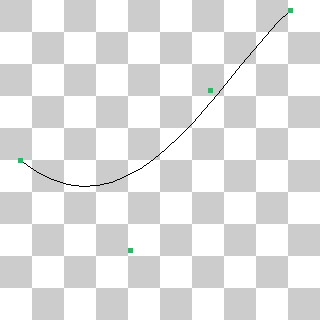
\includegraphics[scale=0.4]{figure/BezierCurve1.png}
    }\quad
    \subfigure[Bezier Curve 2]{
        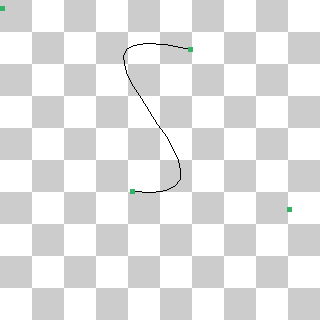
\includegraphics[scale=0.4]{figure/BezierCurve2.png}
    }\quad
    \subfigure[Bezier Curve 3]{
        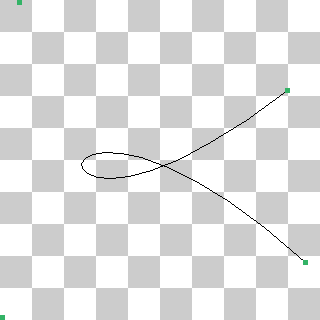
\includegraphics[scale=0.4]{figure/BezierCurve3.png}
    }
    \caption{Bezier Curve的运行结果}
\end{figure}

\end{document}